
All of the protocols were implemented in Java 6 on a server (3GHz AMD processor, 6GB of RAM) running Ubuntu 12.04. These
benchmarks measured latency, the amount of work each device would have to do in the group excluding communication.
\\
For all settings, 2048-bit primes $p$ are used. The same values for SPEKE+ and JPAKE+ were used as in \cite{HaYiChSh15}.
Values for PPK+ were taken from JPAKE+, and values for Dragonfly+ were taken from the NIST cryptographic toolkit (\cite{NIST}).
\\
For groups sizes from 3 to 20 participants, we measure the latency of computation at each round of the protocol. The measurement
was done by repeating the same experiment 100 times and taking the average values. The results are summarized in Figure \ref{fig:results}.


\begin{figure}[h]
    \centering
    \begin{subfigure}[b]{0.5\textwidth}
        \centering
        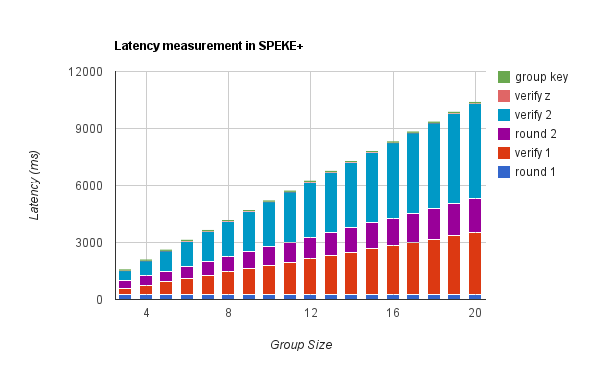
\includegraphics[width=\textwidth]{benchmark/speke.png}
        \caption{SPEKE+ latency results.}
        \label{fig:speke_results}
    \end{subfigure}
    ~
    \begin{subfigure}[b]{0.5\textwidth}
        \centering
        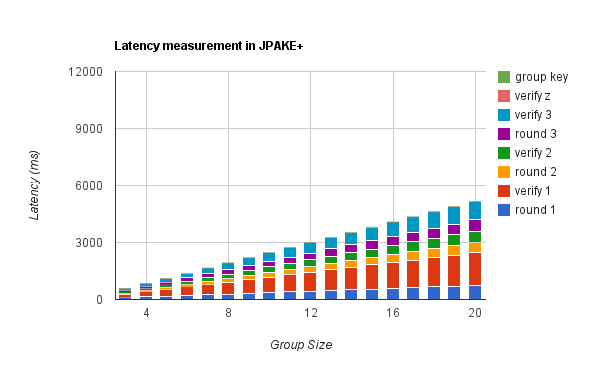
\includegraphics[width=\textwidth]{benchmark/scale_jpake.png}
        \caption{JPAKE+ latency results.}
        \label{fig:jpake_results}
    \end{subfigure}
    \begin{subfigure}[b]{0.5\textwidth}
        \centering
        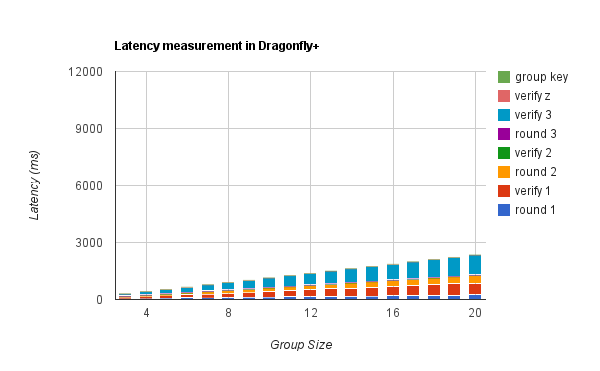
\includegraphics[width=\textwidth]{benchmark/scale_dragon.png}
        \caption{Dragonfly+ latency results.}
        \label{fig:dragon_results}
    \end{subfigure}
    ~
    \begin{subfigure}[b]{0.5\textwidth}
        \centering
        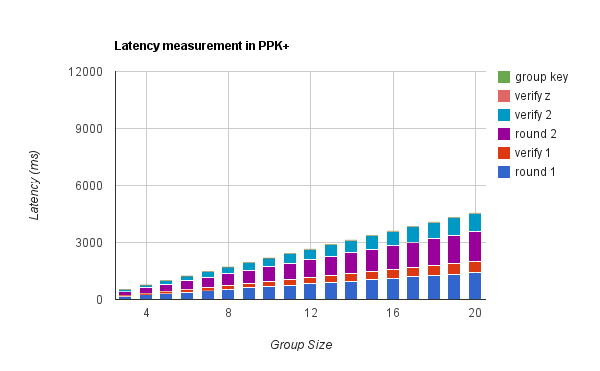
\includegraphics[width=\textwidth]{benchmark/scale_ppk.png}
        \caption{PPK+ latency results.}
        \label{fig:ppk_results}
    \end{subfigure}
    \caption{Latency measurement results for the GPAKE extensions of each of the PAKE protocols.}
    \label{fig:results}
\end{figure}

%\begin{center}
%    \begin{figure}[h]
%        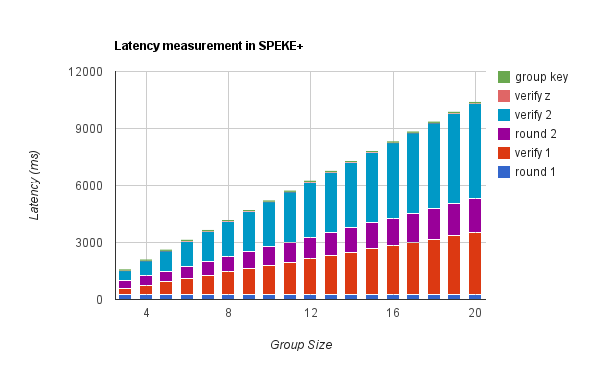
\includegraphics[scale=0.5]{benchmark/speke.png}
%        \caption{SPEKE+ latency results.}
%        \label{fig:speke_results}
%    \end{figure}
%    \begin{figure}[h]
%        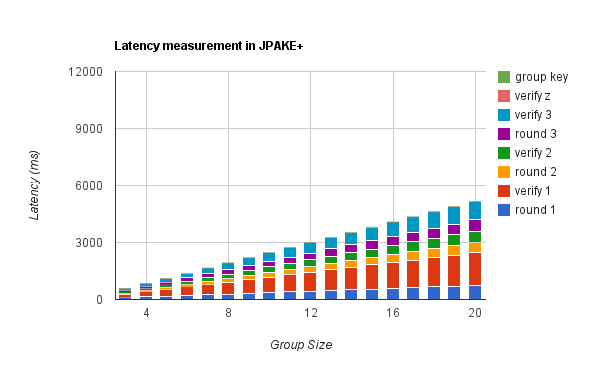
\includegraphics[scale=0.5]{benchmark/scale_jpake.png}
%        \caption{JPAKE+ latency results.}
%        \label{fig:jpake_results}
%   \end{figure}
%    \begin{figure}[h]
%        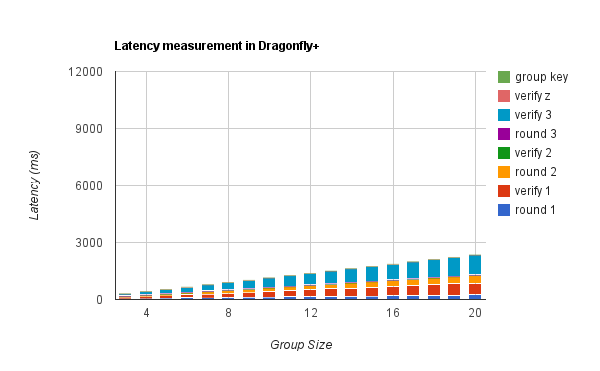
\includegraphics[scale=0.5]{benchmark/scale_dragon.png}
%        \caption{Dragonfly+ latency results.}
%        \label{fig:dragon_results}
%    \end{figure}
%    \begin{figure}[h]
%        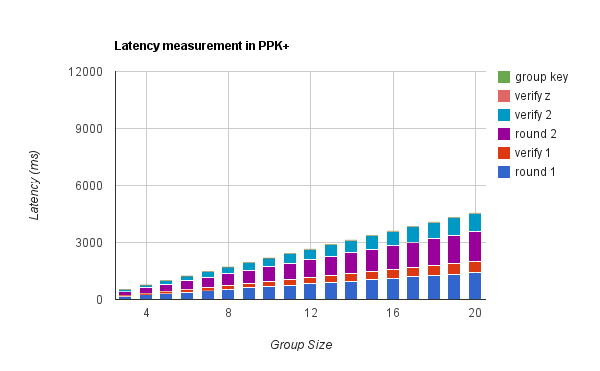
\includegraphics[scale=0.5]{benchmark/scale_ppk.png}
%        \caption{PPK+ latency results.}
%        \label{fig:ppk_results}
%    \end{figure}
%\end{center}

As shown in Figure \ref{fig:results}, the total latency for each member increases linearly with the size of group, regardless of the protocol.
\comment{etc... etc...}

